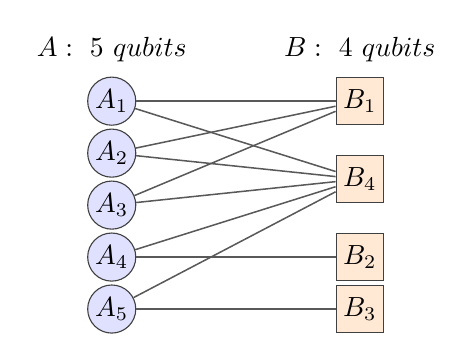
\begin{tikzpicture}[x=1.05cm,y=0.66cm,
  va/.style={circle,draw=black!75,fill=blue!12,minimum size=6mm,inner sep=1pt},
  vb/.style={rectangle,draw=black!75,fill=orange!17,minimum size=6mm,inner sep=1pt}]
\node[va] (a1) at (0,4) {$A_1$};
\node[va] (a2) at (0,3) {$A_2$};
\node[va] (a3) at (0,2) {$A_3$};
\node[va] (a4) at (0,1) {$A_4$};
\node[va] (a5) at (0,0) {$A_5$};
\node[vb] (b1) at (3,4) {$B_1$};
\node[vb] (b2) at (3,1) {$B_2$};
\node[vb] (b3) at (3,0) {$B_3$};
\node[vb] (b4) at (3,2.5) {$B_4$};
\foreach \a/\b in {a1/b1,a1/b4,a2/b1,a2/b4,a3/b1,a3/b4,a4/b2,a4/b4,a5/b3,a5/b4}
  \draw[black!65,line width=0.55pt] (\a) -- (\b);
\node at (0,5) {$A:\ 5\ \text{qubits}$};
\node at (3,5) {$B:\ 4\ \text{qubits}$};
\end{tikzpicture}
